\documentclass[a4paper,papersize,25pt,slide,dvipdfmx]{jsarticle}
\usepackage{hytexconf16} % personal settings
\usepackage[deluxe]{otf}
%\usepackage{plext,plextarray}
\usepackage{newpxtext,newpxmath}
\usepackage{graphicx,xcolor}
\usepackage{overpic,pict2e}
\usepackage{tikz,tcolorbox}
\usepackage[colorlinks=true]{hyperref}
\usepackage{pxjahyper}
\renewcommand{\maybeblue}{\color{blue!40!black}}
%\AtBeginDvi{\special{pdf:mapfile otf-kozuka-pr6n.map}}
\AtBeginDvi{\special{pdf:mapfile kozukapr6n.map}}
\title{\TeX\ Live 2016の新しい\pLaTeX}
\author{山下 弘展(Hironobu Yamashita)\\
        Twitter: \href{http://twitter.com/aminophen}{@aminophen}}
\date{2016年11月5日\\\TeX ユーザの集い2016}
\begin{document}
\maketitle

%%%%%%%%%%%%%%%%%%%%%%%%%%%%%%%%%%%%%%%%%%%%%%%%%%
% INTRO
\SLIDEBEGIN{2}
@SLIDEFIRST
\EMPH{\TeX\ Live 2015}(最終版)
\begin{flushleft}
\footnotesize\baselineskip10pt\ttfamily
\begingroup
\catcode`\~=13\catcode`\ =13\def~{\\}\def {\ }%
\catcode`\|=0\relax\catcode`\$=12\relax\catcode`\\=12\relax
$ platex x~%
This is e-pTeX, Version 3.14159265-p3.6-141210-2.6 (utf8.euc)~%
 (TeX Live 2015) (preloaded format=platex)~%
 restricted \write18 enabled.~%
entering extended mode~%
(/usr/local/texlive/2015/texmf-dist/tex/latex/tools/x.tex~%
pLaTeX2e <2006/11/10> (based on LaTeX2e <2016/03/31> patch level 0)~%
Babel <3.9q> and hyphenation patterns for 81 language(s) loaded.
|endgroup
\end{flushleft}
\vfill
@SLIDESECOND
\EMPH{\TeX\ Live 2016}(\today 現在の最新版)
\begin{flushleft}
\footnotesize\baselineskip10pt\ttfamily
\begingroup
\catcode`\~=13\catcode`\ =13\def~{\\}\def {\ }%
\catcode`\|=0\relax\catcode`\$=12\relax\catcode`\\=12\relax
$ platex x~%
This is e-pTeX, Version 3.14159265-|COLOREMPH{p3.7}-160201-2.6 (utf8.euc)~%
 (TeX Live |COLOREMPH{2016}) (preloaded format=platex)~%
 restricted \write18 enabled.~%
entering extended mode~%
(/usr/local/texlive/2016/texmf-dist/tex/latex/tools/x.tex~%
pLaTeX2e |COLOREMPH{<|pfmtversion>}
(based on LaTeX2e <|fmtversion> patch level 3)~%
Babel <3.9r> and hyphenation patterns for 83 language(s) loaded.
|endgroup
\end{flushleft}
@SLIDELAST
\SLIDEEND

%%%%%%%%%%%%%%%%%%%%%%%%%%%%%%%%%%%%%%%%%%%%%%%%%%
% 1
\SLIDEBEGINx{4}
\SECTION{\LaTeX のこれまで}
@SLIDEFIRST
% http://www.xent.com/FoRK-archive/feb98/0307.html
% http://www.dm.ufscar.br/~sadao/latex/tex-history.php?lang=en
\begin{tabular}{ll}
  1985.08 & \LaTeX~2.09 (Leslie Lamport)
\end{tabular}
@SLIDEFIRSTx
\begin{tabular}{ll}
  \phantom{1985.08} & ↑これがLamport氏による最後の版\footnotemark
\end{tabular}
\footnotetext{\LaTeX~2.09の呼称はあとになってから定着したもの}
\begin{tcolorbox}[sharp corners,colback=blue!5!white,%
                  colframe=blue!40!black,boxrule=1pt]
  \EMPH{1989.08.21} (TUG meeting, Stanford)\\
  Lamport氏が,以降の\LaTeX のメンテナンスと開発を\LaTeX~3
  Teamに引き継ぐことに同意
\end{tcolorbox}
\begin{tabular}{ll}
  \EMPH{1994.06} & \COLOREMPH{\LaTeXe\ (\LaTeX~3 Team)}
\end{tabular}
\begin{quote}\small
\begin{itemize}
  \item スタイルファイル → 文書クラスとパッケージへ分離 \\
  \begin{itemize}
    \item[-] \verb+\documentstyle+から\verb+\documentclass+へ
    \item[-] \verb+\usepackage+の新設
  \end{itemize}
  \item NFSS2 (New Font Selection Scheme release 2, 1993)を採用
\end{itemize}
\vfill\hfill → これらはもはや現在では「あたりまえ」となっている.
\end{quote}
@SLIDESECOND
\begin{tabular}{ll}
  1994.06 & \LaTeXe\ (\LaTeX~3 Team)
\end{tabular}
\begin{quote}
現在の“あたりまえ”が出来た一方で,不都合な点も
\begin{itemize}\small
  \item オリジナルの\TeX の資源不足
  \item 式による計算,デバッグ機能の需要
\end{itemize}
\end{quote}
\begin{tabular}{ll}
  \EMPH{1998.02} & \COLOREMPH{\eTeX\ version 2.0}\footnotemark\
                   (The \NTS\ Team)
\end{tabular}
\footnotetext{\eTeX\ Manual
              (\texttt{\$TEXMF/doc/etex/base/etex\_man.pdf})}
\begin{quote}
\begin{itemize}\small
  \item レジスタが256個から32768個へ
  \item \verb+\dimexpr+などの計算用のprimitive
  \item デバッグ用のprimitiveを多数実装
\end{itemize}
\end{quote}
\begin{tabular}{ll}
  \EMPH{2003.12} & \LaTeXe の\eTeX での利用を\EMPH{推奨}\footnotemark\
                   ← 必須とはしない
\end{tabular}
\footnotetext{\LaTeX\ News Issue~16
              (\texttt{\$TEXMF/source/latex/base/ltnews16.tex})}
@SLIDETHIRD
\begin{tabular}{ll}
  1985.08 & \LaTeX~2.09 (Leslie Lamport) \\
\end{tabular}
\begin{tabular}{ll}
  1994.06 & \LaTeXe\ (\LaTeX~3 Team) \\
\end{tabular}
\begin{quote}
\begin{itemize}
  \item カーネルの変更は最小限にとどめる
  \item 互換性を損なう修正は\file{fixltx2e}パッケージで提供
\end{itemize}
\end{quote}
@SLIDETHIRDx
\begin{tcolorbox}[sharp corners,colback=red!5!white,%
                  colframe=red!40!black,boxrule=1pt]
\EMPH{\large いつまでたってもデフォルトが“良く”ならない}
\begin{itemize}
  \item[-] \eTeX 拡張を利用したければ\file{etex}パッケージを利用
  \item[-] 段組み時のフロートの順序
  \item[-] \verb+\addpenalty+や\verb+\setlength+の定義
  \item[-] フロート環境内の最初の単語のハイフネーション
  \item[] ... etc.
\end{itemize}
\end{tcolorbox}
@SLIDEFOURTH
\begin{center}↓\end{center}
\begin{tabular}{ll}
  \EMPH{2015.01} & \COLOREMPH{\LaTeXe\ 2015/01/01大規模改修}\footnotemark
\end{tabular}
\footnotetext{\TeX\ Live 2015以降に反映;
\href{http://oku.edu.mie-u.ac.jp/tex/mod/forum/discuss.php?d=1558}
     {怒涛のChange History (forum:1558)}}
\begin{quote}
\begin{itemize}
  \item \eTeX 拡張が利用可能ならば活用
  \item 修正が必要な場合はカーネルを直接修正する
  \item 過去のカーネルをエミュレートする\file{latexrelease}パッケージの新設
  \item \file{fixltx2e}パッケージの廃止
\end{itemize}
\vfill\hfill → 2016年11月現在,\LaTeXe\ 2016/03/31 Patch level 3
\end{quote}
@SLIDELAST
\SLIDEEND

%%%%%%%%%%%%%%%%%%%%%%%%%%%%%%%%%%%%%%%%%%%%%%%%%%
% 2
\SLIDEBEGINx{4}
\SECTION{\pLaTeX のこれまで}
@SLIDEFIRST
\begin{tabular}{ll}
1980s   & \pLaTeX~2.09 (ASCII Corporation) \\
\EMPH{1995.11} & \EMPH{\pLaTeXe\ (ASCII Corporation)} \\
2006.11 & アスキーによる現時点で最後の版
\end{tabular}
\begin{quote}
\pTeX は日本ローカルのまま,UTF-8入力不可,\eTeX 拡張なし
\begin{itemize}\small
\item te\TeX ベースのptetexや後継のptexliveによる配布
\item 入力文字コードとしてUTF-8に対応
\item \eTeX\ + \pTeX\ = \epTeX の登場
\item 内部コードをUnicode化した\upTeX,\eupTeX の登場
\end{itemize}
\end{quote}
@SLIDEFIRSTx
@SLIDESECOND
\begin{tabular}{ll}
\EMPH{2010.05} & \COLOREMPH{\pLaTeXe が\pTeX とともに\TeX\ Liveへ収録} \\
2011.01 & \epTeX が\TeX\ Liveに収録される \\
        & \pLaTeXe の既定エンジンが\epTeX に \\
2011.08 & \upLaTeXe が\upTeX/\eupTeX とともに\TeX\ Liveへ収録 \\
\end{tabular}
\begin{quote}
→ \pTeX が\TeX\ Liveと一体で開発可能(\pLaTeX だけ取り残される)
\end{quote}
@SLIDETHIRD
\begin{tabular}{ll}
1980s   & \pLaTeX~2.09 (ASCII Corporation) \\
\EMPH{1995.11} & \EMPH{\pLaTeXe\ (ASCII Corporation)} \\
2006.11 & アスキーによる現時点で最後の版
\end{tabular}
\begin{tcolorbox}[sharp corners,colback=blue!5!white,%
                  colframe=blue!40!black,boxrule=1pt]
\EMPH{2016.01.06} (devel mailing list) \\
日本語\TeX 開発コミュニティが\pLaTeXe をforkし,メンテナンス
開始 = コミュニティ版\pLaTeX
\end{tcolorbox}
@SLIDETHIRDx
\smallskip
日本語\TeX 開発コミュニティ(Japanese \TeX\ Development Community)
… 旧p\TeX-mlの後継としての開発者向けメーリングリスト\par
   \hfill 日本語まわりの\TeX 環境の整備(\pTeX 系にかぎらず開発全般)
\begin{quote}
\begin{itemize}
  \item \url{https://texjp.org}
  \item \url{https://github.com/texjporg}
\end{itemize}
\end{quote}
@SLIDEFOURTH
\begin{tabular}{ll}
2016.06 & \TeX\ Forumにて\EMPH{コミュニティ版\pLaTeX 発表}\footnotemark
\end{tabular}
\footnotetext{%
\href{http://oku.edu.mie-u.ac.jp/tex/mod/forum/discuss.php?d=1934}
     {\pLaTeX と\upLaTeX のコミュニティ版(2016/05/07) (forum:1934)}}
\begin{quote}
\begin{itemize}
\item \TeX\ Live 2016以降(含W32\TeX)\footnote{より正確にはW32\TeX では5月2日,\TeX\ Live 2016 pretestでは5月10日以降.}に反映
\item \upLaTeX もコミュニティ版\pLaTeX ベースに
\item ライセンスはBSD 3-Clause(アスキー版\pLaTeXe と同じ)
\end{itemize}
\end{quote}
@SLIDELAST
\SLIDEEND

%%%%%%%%%%%%%%%%%%%%%%%%%%%%%%%%%%%%%%%%%%%%%%%%%%
% 3
\SLIDEBEGIN{3}
\SECTION{コミュニティ版\pLaTeX の目的}
@SLIDEFIRST
最優先課題:
\begin{center}
2013年の\pTeX の仕様変更による副作用への対処\par
(脚注の合印前後に入る不自然な\verb+\xkanjiskip+アキ問題)
\end{center}
@SLIDESECOND
もっと広げると
\begin{center}\Large
\EMPH{\pTeX の仕様変更・\LaTeX の仕様変更で\\
不都合が生じないようにメンテナンス}
\end{center}
@SLIDETHIRD
\smallskip
\begin{quote}
\begin{itemize}
\item エンジンである\pTeX や\epTeX
      は,\TeX\ Liveのリポジトリで修正・変更されている.
\item \LaTeX も2015年以降,どんどん変わっている.
\item この流れから\pLaTeX だけ取り残されるのは嬉しくない.
\end{itemize}
\end{quote}
@SLIDELAST
\SLIDEEND

%%%%%%%%%%%%%%%%%%%%%%%%%%%%%%%%%%%%%%%%%%%%%%%%%%
% 4
\SLIDEBEGIN{1}
\SECTION{組版結果にかかわる\pLaTeX の修正・仕様変更}
@SLIDEFIRST
\begin{quote}
\begin{itemize}
  \item 脚注番号(合印)前後のアキ:\pTeX への追随
  \item 表組前後のアキ:\pTeX への追随
  \item 下線前後のアキ:仕様変更
  \item 脚注番号(合印)前後のベタ組:仕様変更
  \item 合印直後の改行を許容:仕様変更
  \item 8-bit font encodingの欧文文字前後の四分アキ:仕様変更
\end{itemize}
\end{quote}
@SLIDELAST
\SLIDEEND

\SLIDEBEGINx{3}
\SUBSECTION{脚注番号(合印)前後のアキ:\pTeX への追随}
@SLIDEFIRST
@SLIDEFIRSTx
\begin{overpic}[width=.8\textwidth]{demo/demo01-2012.pdf}
 \linethickness{2pt}
 \put(95,0){
\includegraphics[scale=1]{img/snowman0-sourcehansans.pdf}}
 \put(100,15){\vector(-5,2){30}}
 \put(100,28){\begin{minipage}{6zw}\COLOREMPH{ここに注目!}\end{minipage}}
\end{overpic}
@SLIDESECOND
@SLIDESECONDx
\begin{overpic}[width=.8\textwidth]{demo/demo01-2013.pdf}
 \linethickness{2pt}
 \put(95,0){
\includegraphics[scale=1]{img/snowman0-yuosx.pdf}}
 \put(100,28){\begin{minipage}{6zw}\COLOREMPH{不自然なアキ}\end{minipage}}
\end{overpic}\par\vfill\hfill
{\large 2013年の\pTeX の仕様変更\footnote{%
\href{http://oku.edu.mie-u.ac.jp/tex/mod/forum/discuss.php?d=913}
{数式の前後の四分アキ (forum:913)}}に起因する\verb+\xkanjiskip+アキ}
@SLIDETHIRD
\begin{overpic}[width=.8\textwidth]{demo/demo01-2016.pdf}
 \linethickness{2pt}
 \put(95,0){
\includegraphics[scale=1]{img/snowman0-sourcehansans.pdf}}
 \put(100,28){\begin{minipage}{6zw}\COLOREMPH{元に戻った!}\end{minipage}}
\end{overpic}\par\vfill
{\pLaTeX カーネルで\texttt{\char92\char64makefnmark}を
再定義することにより,従来の挙動を取り戻した}\vfill
@SLIDELAST
\SLIDEEND

\SLIDEBEGINx{5}
\SUBSECTION{表組前後のアキ:\pTeX への追随}
@SLIDEFIRST
@SLIDEFIRSTx
\begin{overpic}[width=.8\textwidth]{demo/demo02-2012.pdf}
 \linethickness{2pt}
 \put(95,0){
\includegraphics[scale=1]{img/snowman0-sourcehansans.pdf}}
 \put(90,10){\vector(-1,2){9}}
 \put(10,10){\vector(1,2){9}}
 \put(100,28){\begin{minipage}{6zw}\COLOREMPH{ここに注目!}\end{minipage}}
\end{overpic}
@SLIDESECOND
@SLIDESECONDx
\begin{overpic}[width=.8\textwidth]{demo/demo02-2013.pdf}
 \linethickness{2pt}
 \put(95,0){
\includegraphics[scale=1]{img/snowman0-yuosx.pdf}}
 \put(100,28){\begin{minipage}{6zw}\COLOREMPH{アキが入る}\end{minipage}}
\end{overpic}\par
{\large これもやはり,2013年の\pTeX の仕様変更に起因する}
@SLIDETHIRD
\begin{overpic}[width=.8\textwidth]{demo/demo02-2016.pdf}
 \linethickness{2pt}
 \put(95,0){
\includegraphics[scale=1]{img/snowman0-sourcehansans.pdf}}
 \put(100,28){\begin{minipage}{6zw}\COLOREMPH{元に戻った!}\end{minipage}}
\end{overpic}\par
{\large → \pLaTeX で\texttt{tabular}環境を再定義し,従来の挙動へ復帰}
@SLIDEFOURTH
\begin{tikzpicture}
 \node[color=blue,opacity=.7] at (0,0)
 {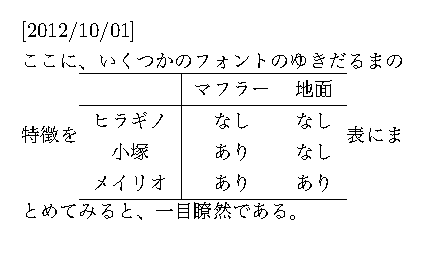
\includegraphics[width=.8\textwidth]{demo/demo02-2012.pdf}};
 \node[color=blue,opacity=.7] at (5,1) {2012年};
 \node[color=red,opacity=.7] at (0,0)
 {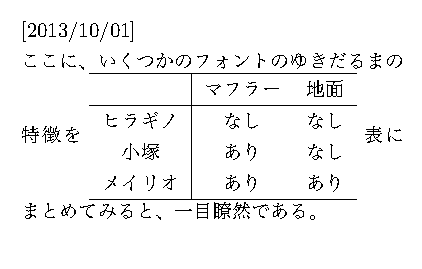
\includegraphics[width=.8\textwidth]{demo/demo02-2013.pdf}};
 \node[color=red,opacity=.7] at (5,-1) {2013年};
\end{tikzpicture}
\pTeX が変われば(\pLaTeX は変わらなくても)出力は変わってしまう
@SLIDEFOURTHx
@SLIDEFIFTH
\par →
\EMPH{\pTeX を変える場合は,\pLaTeX も必要に応じて変えなければならない}
@SLIDELAST
\SLIDEEND

\SLIDEBEGINx{2}
\SUBSECTION{下線前後のアキ:\pLaTeX の仕様変更}
@SLIDEFIRST
@SLIDEFIRSTx
\begin{overpic}[width=.8\textwidth]{demo/demo03-2013.pdf}
 \linethickness{2pt}
 \put(95,0){
\includegraphics[scale=1]{img/snowman0-hiragino.pdf}}
 \put(50,60){\vector(-1,-1){8}}
 \put(100,45){\vector(-1,-1){8}}
 \put(100,28){\begin{minipage}{6zw}\COLOREMPH{下線の前後にアキがある}\end{minipage}}
\end{overpic}\par\vfill
たびたび言及あり\par
奥村晴彦・黒木裕介 著「改訂第6版 \LaTeXe 美文書入門」(2013) p.291,
吉永徹美 著「独習\LaTeXe」(2008) p.110など \vfill
@SLIDESECOND
\begin{overpic}[width=.8\textwidth]{demo/demo03-2016.pdf}
 \linethickness{2pt}
 \put(95,0){
\includegraphics[scale=1]{img/snowman0-meiryo.pdf}}
 \put(100,28){\begin{minipage}{6zw}\COLOREMPH{アキを削除!}\end{minipage}}
\end{overpic}\par
{\large → \pLaTeX カーネルで\verb+\underline+を再定義し,アキを削除}
@SLIDELAST
\SLIDEEND

\SLIDEBEGINx{2}
\SUBSECTION{脚注番号(合印)前後のベタ組:\pLaTeX の仕様変更}
@SLIDEFIRST
@SLIDEFIRSTx
\begin{overpic}[width=.8\textwidth]{demo/demo04-2012.pdf}
 \linethickness{2pt}
 \put(95,0){
\includegraphics[scale=1]{img/snowman0-hiragino.pdf}}
 \put(70,15){\vector(-1,1){10}}
 \put(100,28){\begin{minipage}{6zw}\COLOREMPH{区切り約物の後ろにアキ}\end{minipage}}
\end{overpic}\par\vfill
\file{jsclasses}ではかなり昔から修正済み \vfill
@SLIDESECOND
\begin{overpic}[width=.8\textwidth]{demo/demo04-2016.pdf}
 \linethickness{2pt}
 \put(95,0){
\includegraphics[scale=1]{img/snowman0-meiryo.pdf}}
 \put(100,28){\begin{minipage}{6zw}\COLOREMPH{ベタ組に!}\end{minipage}}
\end{overpic}\par
{\large → \pLaTeX カーネルに\file{jsclasses}と同様のコードを導入\par
\quad (どちらの流儀が“一般的”かは問わない)}
@SLIDELAST
\SLIDEEND

\SLIDEBEGINx{2}
\SUBSECTION{合印直後の改行を許容:\pLaTeX の仕様変更}
@SLIDEFIRST
@SLIDEFIRSTx
\begin{overpic}[width=.8\textwidth]{demo/demo05-2012.pdf}
 \linethickness{2pt}
 \put(95,0){
\includegraphics[scale=1]{img/snowman0-hiragino.pdf}}
 \put(100,10){\vector(-8,3){84}}
 \put(100,33){\begin{minipage}{6zw}\COLOREMPH{「1」と「を」の間は
分割禁止でないはず…}\end{minipage}}
\end{overpic}\par\vfill
行分割してよいはずの場所で改行が起きない\par
→ スカスカの行が出来たり,\texttt{Overfull}警告が出たり… \vfill
@SLIDESECOND
\begin{overpic}[width=.8\textwidth]{demo/demo05-2016.pdf}
 \linethickness{2pt}
 \put(95,0){
\includegraphics[scale=1]{img/snowman0-meiryo.pdf}}
 \put(101,10){\vector(-1,6){6}}
 \put(100,28){\begin{minipage}{6zw}\COLOREMPH{分割可能に!}\end{minipage}}
\end{overpic}\par
{\large → \pLaTeX カーネルを修正し,自然な行組版を可能に}
@SLIDELAST
\SLIDEEND

\SLIDEBEGINx{2}
\SUBSECTION{8-bit font encodingの欧文文字前後の四分アキ}
@SLIDEFIRST
@SLIDEFIRSTx
\begin{overpic}[width=.8\textwidth]{demo/demo06-2012.pdf}
 \linethickness{2pt}
 \put(95,0){
\includegraphics[scale=1]{img/snowman0-hiragino.pdf}}
 \put(45,60){\vector(-1,-1){8}}
 \put(90,60){\vector(-1,-1){8}}
 \put(60,36){\vector(-1,-1){8}}
 \put(100,28){\begin{minipage}{7zw}\COLOREMPH{アクセント文字の
前後に和欧文間空白がない!}\end{minipage}}
\end{overpic}\par\vfill
当時はT1エンコーディングなどが一般的ではなく,
未考慮だったらしい(\file{jsclasses}や\upLaTeX では対処済み)
\vfill
@SLIDESECOND
\begin{overpic}[width=.8\textwidth]{demo/demo06-2016.pdf}
 \linethickness{2pt}
 \put(95,0){
\includegraphics[scale=1]{img/snowman0-meiryo.pdf}}
 \put(100,28){\begin{minipage}{6zw}\COLOREMPH{四分アキあり}\end{minipage}}
\end{overpic}\par
{\large → \pLaTeX でも文字コード128--255に\verb+\xspcode=3+を設定}
@SLIDELAST
\SLIDEEND

%%%%%%%%%%%%%%%%%%%%%%%%%%%%%%%%%%%%%%%%%%%%%%%%%%
% 5
\SLIDEBEGIN{2}
\SECTION{\LaTeX への追随}
@SLIDEFIRST
\begin{quote}
今のところ大事なのはひとつだけ:
\begin{itemize}
  \item 入れ子の強調書体\verb+\eminnershape+の採用
        {\footnotesize ← 要するに\verb+{\em{\em この中}}+}
\end{itemize}
\end{quote}
@SLIDESECOND
\begin{quote}
\begin{itemize}
  \begin{itemize}
    \item[-] デフォルトは従来どおり:
    \verb+\def\eminnershape{\mcfamily \upshape}+\\
    \item[-] カスタマイズ例:
    \verb+\renewcommand{\eminnershape}{\gtfamily \scshape}+\\
  \end{itemize}
\end{itemize}
\end{quote}
\begin{center}
\def\arraystretch{1.8}
\renewcommand{\eminnershape}{\gtfamily \scshape}
\begin{tabular}{c|ccc}\hline
 & 地の文 & 強調 & \COLOREMPH{入れ子の強調} \\ \hline
\LaTeX のデフォルト & \textmc{Roman}
 & \emph{italic} & \emph{\emph{Roman}} \\
\pLaTeX のデフォルト
 & \parbox{3zw}{\centering\textmc{明朝体}\par\textmc{\strut Roman}}
 & \parbox{4zw}{\centering\emph{ゴシック}\par\emph{\strut italic}}
 & \parbox{3zw}{\centering\textmc{明朝体}\par\textmc{\strut Roman}} \\
カスタマイズ
 & \parbox{3zw}{\centering\textmc{明朝体}\par\textmc{\strut Roman}}
 & \parbox{4zw}{\centering\emph{ゴシック}\par\emph{\strut italic}}
 & \parbox{3zw}{\centering\emph{\emph{明朝体}}\par\emph{\emph{\strut Roman}}} \\ \hline
\end{tabular}
\end{center}
@SLIDELAST
\SLIDEEND

%%%%%%%%%%%%%%%%%%%%%%%%%%%%%%%%%%%%%%%%%%%%%%%%%%
% 6
\SLIDEBEGIN{2}
\SECTION{警告やエラーが出る現象への対処}
@SLIDEFIRST
\begin{quote}
\begin{itemize}
  \item 縦組時の\texttt{Overfull}警告の抑制
  \item 縦組で\file{longtable}パッケージが無限ループする現象への対処
  \begin{itemize}
    \item[-] 以上2件は\texttt{\char92\char64makecol}の修正
  \end{itemize}
  \item 縦組で\verb+\AtBeginDocument{\AtBeginDvi}}+のエラーを解消
  \begin{itemize}
    \item[-] \texttt{\char92\char64begindvibox}を常に横組ボックスへ
  \end{itemize}
\end{itemize}
\end{quote}
@SLIDESECOND
\begin{quote}
\file{ascmac}パッケージも修正
\begin{itemize}
  \item \file{pict2e}パッケージと併用するとエラーが出る現象への対処
  \begin{itemize}
    \item[-] 従来は\verb+! Missing number, treated as zero.+などのエラー
  \end{itemize}
  \item pdf\LaTeX などでも利用可能なように拡張
  \begin{itemize}
    \item[-] 従来は\verb+\tbaselineshift+が未定義というエラー
  \end{itemize}
  \item \verb+\keytop+や\texttt{screen}/\texttt{itembox}の角のズレ修正\\

\includegraphics[scale=3]{demo/demo07-2013-crop.pdf} \raisebox{2zh}{→}

\includegraphics[scale=3]{demo/demo07-2016-crop.pdf}
(印刷すると綺麗なはず)
\end{itemize}
\end{quote}
@SLIDELAST
\SLIDEEND

%%%%%%%%%%%%%%%%%%%%%%%%%%%%%%%%%%%%%%%%%%%%%%%%%%
% 7
\SLIDEBEGIN{3}
\SECTION{カーネルの互換性…過去の挙動のエミュレート}
@SLIDEFIRST
\begin{quote}
新しい\pLaTeX には組版上の改良が多数加わりました\par
→ でも,前に書いたソースは“同じ見た目”になってほしい
{\footnotesize (場合もある)}
\end{quote}
@SLIDESECOND
\begin{quote}
そんなときは
\begin{center}
{\Large\EMPH{\file{platexrelease}パッケージ}}
\end{center}
\begin{itemize}
  \item 本家\LaTeX に添付の\file{latexrelease}パッケージの\pLaTeX 版
  \item 日付を指定して読み込むと,その日付の\pLaTeX カーネルを再現 \\
        \verb+  \RequirePackage[2016/03/31]{platexrelease}+\\
        \verb+  \documentclass{jsarticle}+\\
→ 2016/03/31時点の\LaTeXe と\pLaTeXe の組み合わせ
\end{itemize}
\end{quote}
多くの場合には,これで過去の挙動をエミュレートすれば“同じ見た目”
になるはず.
@SLIDETHIRD
\EMPH{ただし:}
\begin{center}
\COLOREMPH{原理的に完全ではない(\pTeX の挙動が変わった場合は,再現不能)}
\end{center}
@SLIDELAST
\SLIDEEND

%%%%%%%%%%%%%%%%%%%%%%%%%%%%%%%%%%%%%%%%%%%%%%%%%%
% 8
\SLIDEBEGIN{3}
\SECTION{\pLaTeX の今後}
@SLIDEFIRST
最大の課題
\begin{center}\large
\EMPH{どのような変更を許容するか}
\end{center}\smallskip
@SLIDESECOND
\begin{quote}
\pTeX の挙動は案外コロコロ変わっている(特に四分アキと和欧文ベースライン補正で顕著)
\begin{itemize}
\item 数式も欧文とみなしてベースラインシフト(2009)
\item 数式周囲の\verb+\xkanjiskip+挿入漏れを解消(2013)
\item 数式内の明示的な\verb+\hbox+ではベースラインシフトを戻す(2016)
\item 数式周囲の\verb+\xkanjiskip+挿入漏れをさらに解消(2017)
\item 縦ディレクションと縦数式ディレクションの区別(2017)
\end{itemize}
\end{quote}
@SLIDETHIRD
\begin{quote}
いずれもアスキーによる最後の\pLaTeX~2006/11/10より\EMPH{後}の変更\par
→ これによって\COLOREMPH{\pLaTeX の挙動が変わっている(いた)!}\par
{\small この事態に対する指摘が6年間で極端に少なかったのはなぜ?}
\end{quote}
@SLIDELAST
\SLIDEEND

\SLIDEBEGIN{4}
\SUBSECTION{\pLaTeX の変更をどこまで許容するか}
@SLIDEFIRST
\pTeX/\epTeX の変化に由来する\pLaTeX の変化に「気づいていない」?\par
組版結果の変化に対して寛容?\par\medskip
@SLIDESECOND
一つの主張:
\begin{center}
「\pLaTeX カーネルは\EMPH{安定}であるべき」
\end{center}
言うのは簡単,では具体的には?
@SLIDETHIRD
\begin{quote}
\begin{itemize}
\item 出力が変わらないこと?
\item コードに触らないこと?
\end{itemize}
コードに触ればバグもつきもの.\par
でも触らないで不都合な挙動を残すのも親切とは思えない.
\end{quote}
@SLIDEFOURTH
私の立場:
\begin{quote}
\begin{itemize}
\item バグが入ることも覚悟で\EMPH{コードを変更}\quad
{\small ← \LaTeX もそうやっているし.}
\item バグや不都合の報告が来たら\EMPH{速攻で直す}or戻す!
\end{itemize}
\end{quote}
@SLIDELAST
\SLIDEEND

\SLIDEBEGINx{3}
\SUBSECTION{「変える」ことによる安定性}
@SLIDEFIRST
大事なことなのでもう一度,私の立場:
\begin{quote}
\begin{itemize}
\item バグが入ることも覚悟で\EMPH{コードを変更}
\item バグや不都合の報告が来たら\EMPH{速攻で直す}or戻す!
\end{itemize}
\end{quote}
@SLIDEFIRSTx
\begin{quote}
まずは認識のすりあわせ(立場の明言は大事です)
\end{quote}
\begin{itemize}
\item 「\pLaTeX は極力いじらない」ではなく \\
      「その時点の\pTeX\ (\epTeX)と\LaTeX の上に構築された状態」を考える
\begin{itemize}
\item[-] \pTeX (または\epTeX)も\LaTeX も変わっているのに,その上で
動作する\COLOREMPH{\pLaTeX の出力が変わらないのを期待するのは酷}だよね.
\item[-] \pTeX (または\epTeX)を改良するのであれば,\pLaTeX も
改良していくのが自然.(ダブルスタンダードの防止)
\end{itemize}
\item では,\pLaTeX 標準クラス(\file{jarticle},\file{tarticle}など)は?
\end{itemize}
@SLIDESECOND
\begin{quote}
もちろん,バグが入らないように努力する(→ 後述)\par
でも完璧ではない.大事なのは:
\end{quote}
\begin{center}
バグを入れないことよりも,\EMPH{入りうるバグの影響の最小化}
\end{center}
@SLIDESECONDx
@SLIDETHIRD
\begin{quote}
たとえば:
\begin{itemize}
  \item \TeX\ Liveの年度終盤には大きな変更を入れない
  \begin{itemize}
    \item[-] frozenになってからでは最大2ヶ月にわたり不都合が続く.
  \end{itemize}
  \item 入ってしまったバグへの対症療法をあらかじめ準備
  \begin{itemize}
    \item[-] これは\file{platexrelease}パッケージの仕事.
  \end{itemize}
\end{itemize}
\end{quote}
@SLIDELAST
\SLIDEEND

\SLIDEBEGINx{3}
\SUBSECTION{バグを入れない努力:実験的\pLaTeX}
@SLIDEFIRST
みなさんも「開発版\pLaTeX」をすぐにテストできます!\par
@SLIDEFIRSTx
@SLIDESECOND
@SLIDESECONDx
\begin{center}
\COLOREMPH{\file{exppl2e}パッケージ}\footnote{\file{expl3}パッケージ
や\file{fixltx2e}パッケージをもじった命名}(EXPerimental PLatex2E)
\end{center}
@SLIDETHIRD
\begin{center}
\COLOREMPH{\file{exppl2e}パッケージ}(EXPerimental PLatex2E)
\end{center}
“おまじない”は\verb+\RequirePackage{exppl2e}+
\begin{quote}
\begin{itemize}
\item 任意のファイルの冒頭,あるいは
\item \TeX から見つかる任意の場所に用意した\file{platex.cfg}ファイル
\end{itemize}
\end{quote}
に書くと,テスト版\pLaTeXe (と実質的に同じもの)が動作する.\par
\begin{quote}
\verb+  \RequirePackage{exppl2e}+\\
\verb+  \documentclass{jsarticle}+\\
\verb+  …+
\end{quote}
\begin{quote}
これで,「フォーマット作成って何?」な人でも安心. \par
(もちろん,GitHub -- \url{https://github.com/texjporg/platex}を
見ていただけるともっと嬉しい.)
\end{quote}
@SLIDELAST
\SLIDEEND

\SLIDEBEGINx{5}
\SUBSECTION{具体的なテスト内容(本日,2016年11月5日現在)}
@SLIDEFIRST
@SLIDEFIRSTx
\begin{quote}
\begin{itemize}
\item “アクセント文字パッチ”
\item “\verb+\strutbox+パッチ”
\item \epTeX の“FAM256パッチ”の活用(GitHubのみで配布中)
\end{itemize}\smallskip
組版に大きくかかわるのは最初の2つ.\par\hfill
{\small ちなみに,これらは現行のLua\TeX-jaでも同様らしい.}\par
\medskip
{\small ※FAM256パッチを活用すれば,数式ファミリを従来の16個から
256個まで増やせる.\par
→ \verb+\DeclareMathAlphabet+がたくさんあっても大丈夫}
\end{quote}
@SLIDESECOND
\begin{itemize}
\item “アクセント文字パッチ”の例:\verb+\AA+の出力
\end{itemize}
@SLIDESECONDx
\verb+  \documentclass{tarticle}+\\
\verb+  \begin{document}+\\
\verb+  $1\,\mathrm{nm}$の$1/10$を表す長さの単位は、+\\
\verb+  オングストローム(\AA)と書きます。+\\
\verb+  \end{document}+
@SLIDETHIRD
\begin{quote}
\centering
\raisebox{170pt}{現状}
\begin{overpic}[scale=1.1]{demo/exp01-2016.pdf}
 \linethickness{2pt}
%\put(-50,0){
\includegraphics[scale=1]{img/snowman0-hiragino.pdf}}
 \put(-8,43){\vector(1,0){12}}
 \put(-50,45){\begin{minipage}{8zw}\COLOREMPH{OT1 encodingのアクセント合成文字が変になる}\end{minipage}}
\end{overpic}\hspace{20pt}
\begin{overpic}[scale=1.1]{demo/exp01-2017.pdf}
 \linethickness{2pt}
% \put(40,0){
\includegraphics[scale=1]{img/snowman0-meiryo.pdf}}
 \put(35,43){\vector(-1,0){20}}
 \put(40,55){\begin{minipage}{8zw}\EMPH{一度はカーネルに修正を加えたが,副作用のため現在テスト段階}\end{minipage}}
\end{overpic}
\raisebox{170pt}{修正案}
\end{quote}
@SLIDEFOURTH
\begin{itemize}
\item “\verb+\strutbox+パッチ”の例:\file{amsmath}のalignment (\verb+&+)と数式番号
\end{itemize}
@SLIDEFOURTHx
\verb|  \documentclass{tarticle}|\\
\verb|  \usepackage{amsmath}|\\
\verb|  \begin{document}|\\
\verb|  align環境\texttt{\&}が1つ|\\
\verb|  \begin{align}|\\
\verb|    a_1 &= b_1+c_1\\|\\
\verb|    a_2 &= b_2+c_2-d_2|\\
\verb|  \end{align}|\\
\verb|  align環境\texttt{\&}なし|\\
\verb|  \begin{align}     a_1=b_1+c_1  \end{align}|\\
\verb|  比較用のequation環境|\\
\verb|  \begin{equation}  a_1=b_1+c_1  \end{equation}|\\
\verb|  \end{document}|
@SLIDEFIFTH
\begin{quote}
\hfill 現状 \hfill 修正案 \hfill \hfill \par
\centering
\begin{overpic}[scale=.75]{demo/exp02-2016.pdf}
 \put(0,5){\color{green!50!black}\vector(1,0){80}}
 \put(15,21){\COLOREMPH{数式番号が揃わない}}
 \put(50,12){\color{green}\vector(1,0){20}}
\end{overpic}\hspace{5pt}
\begin{overpic}[scale=.75]{demo/exp02-2017.pdf}
 \put(0,5){\color{green!50!black}\vector(1,0){80}}
 \put(20,21){\EMPH{副作用がないか調査中}}
\end{overpic}
\end{quote}
@SLIDELAST
\SLIDEEND

%%%%%%%%%%%%%%%%%%%%%%%%%%%%%%%%%%%%%%%%%%%%%%%%%%
% finale
\SLIDEBEGIN{2}
\SECTION{まとめ}
@SLIDEFIRST
\begin{quote}
\begin{itemize}
  \item \pLaTeX は2016年以降,コミュニティ版になった
  \item 組版の改善,エラーや警告の解消など
  \item 互換性を\file{platexrelease}パッケージで極力サポート
  \item テスト版\pLaTeX =\file{exppl2e}パッケージへのご協力を
  \item これからは,\pTeX/\epTeX と\LaTeX に追随した\pLaTeX の開発を
  \begin{itemize}
    \item[-] 2017年頭には「\LaTeX は\eTeX 拡張を必須とする」そうです
  \end{itemize}
\end{itemize}
\end{quote}
@SLIDESECOND
\begin{center}
\GOSEICHO
\leavevmode

\includegraphics[scale=1.2]{img/snowman0-meiryo.pdf}\par
Happy \pLaTeX ing!
\end{center}
@SLIDELAST
\SLIDEEND

\end{document}
